\begin{frame}{Related works}{Non blockchain-based}
    \setbeamercovered{transparent}
    \begin{itemize}
        \onslide<1->{\item[1.]US open data portal
              \begin{itemize}
                  \uncover<2->{\item since 2009;}
                        \uncover<3->{\item provides a number of 229,371 data sets in various formats and related to many fields.}
                        %  such as agriculture, ecosystems, education, energy, finance, health, natural disasters, science, and research.}
              \end{itemize}
              }
              \pause
              \pause
              \pause
              \onslide<4->{\item[2.]Ho Chi Minh open data portal
              \begin{itemize}
                  \uncover<5->{\item since 2017;}
                        %   The portal is expected to have integration with some important databases including medical, education, invest, environment, etc.}
                        \uncover<6->{\item still thin in the content due to lacking data sets.}
              \end{itemize}
              }
    \end{itemize}
\end{frame}
\begin{frame}{Related works}{Blockchain-based}
    \begin{itemize}
        \item[3.]Vienna open data portal
              \setbeamercovered{transparent}
              \begin{itemize}
                  \uncover<2->{\item called "Data Notarization Blockchain" in 2018;}
                        %   Austria government has applied the blockchain technology to the open data portal of Vienna and successfully demonstrated under a project named ``Data Notarization Blockchain'' in 2018.}
                        \uncover<3->{\item uses public blockchain.}
                        % Once a contributor publishes a data set, a checksum of it will be stored on the public blockchain network for validating the content of the data.}
              \end{itemize}

    \end{itemize}
    \uncover<4->{
        \begin{figure}
            \centering
            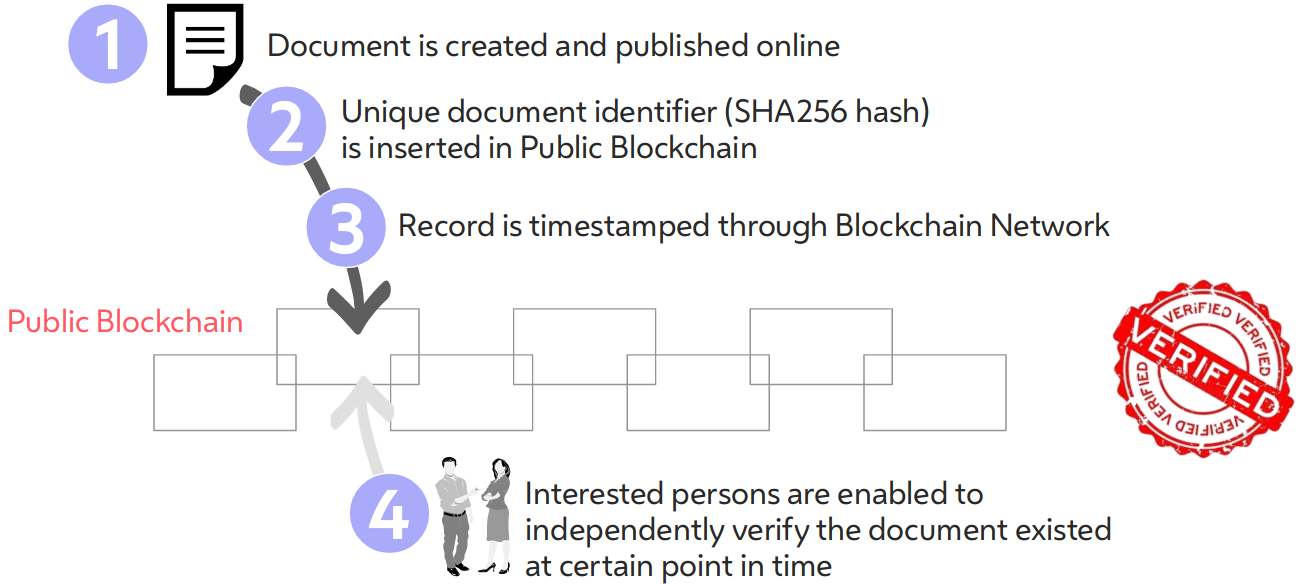
\includegraphics[width=.9\textwidth,height=.4\textwidth]{img/ViennaBc.png}
            % \caption{Vienna Blockchain notarization solution.}
            % \label{fig:arOv}
        \end{figure}}
\end{frame}